\section{Weierstrass and the Monster of Mathematical Rigor: From Infinitesimals to Nowhere-Differentiable Functions (1872)}  

\subsection{The Last Infinitesimal Holdouts}

By the mid-19th century, mathematics had undergone a radical transformation.

Riemann had redefined integration. Cauchy had formalized limits. Analysis was growing teeth—and yet, something ghostly still lingered.

Despite all the progress, infinitesimals hadn’t been fully exorcised. They clung to the edges of calculus like fog on a cleaned window: mostly gone, but still present enough to smudge the view. For centuries, mathematicians had used them freely, intuitively—leaning on them like a rickety ladder—without ever agreeing on what they were. It worked, but only if you didn’t ask too many questions.

But in a world where even the act of integrating needed a microscope and a manifold, intuition was no longer enough.

And not everyone was buying it.

\textbf{Enter George Berkeley.} In 1734—long before Riemann, Cauchy, or Weierstrass—Berkeley dropped the equivalent of a philosophical roast on the foundations of calculus. In his pamphlet \emph{The Analyst}, he famously ridiculed infinitesimals as the “ghosts of departed quantities”—a line so iconic it might as well have trended on Enlightenment Twitter.

And he had a point. Mathematicians had been using \( dx \) and \( dy \) like mystical incantations—producing valid results through dubious logic. The results worked. The reasoning didn’t.

Even after Riemann gave us a way to integrate without infinitesimals, the problem hadn’t disappeared. Because the real question wasn’t just how to add things up. It was this:

\begin{quote}
What is a function, really? And how bad can it get?
\end{quote}

That’s where Weierstrass comes in.

While Riemann had expanded the universe of integrable functions, Weierstrass revealed that this universe was darker—and more twisted—than anyone had imagined. It wasn’t just that some functions couldn’t be integrated. It was that some functions couldn’t even be \emph{differentiated anywhere}, not even once.

The monsters had arrived.

And they didn’t care about your intuition.


\subsection{Enter Weierstrass: The Mathematical Puritan}  

Long before calculus was formalized, Eudoxus had already laid down a way to handle the infinite — without ever invoking it directly. His method?  
\textbf{Compare everything. Measure nothing.}  

Instead of calculating irrational quantities or infinitesimals, Eudoxus defined equality and order purely in terms of how two magnitudes behaved when scaled by whole numbers. If one ratio consistently stayed larger or smaller than another, no matter how many times you multiplied them, then you knew something meaningful — even if you couldn’t measure it.

He applied this logic to lines, areas, and volumes — taming irrational lengths like \( \sqrt{2} \) and allowing geometry to proceed rigorously, even when the quantities themselves were unknowable.  

What Eudoxus did for simple shapes and magnitudes, **Weierstrass would eventually do for general functions.**

Fast forward two thousand years.

Someone had to finish the job and make sure calculus was completely ghost-proof. That someone was Karl Weierstrass, a man who looked at infinitesimals and said,  

\begin{quote}
    \textit{"This is nonsense. We're burning it all down."}
\end{quote}

Weierstrass didn’t invent limits, but he turned them into an ironclad mathematical fortress. While Eudoxus had avoided irrational numbers by comparing magnitudes, and Cauchy had tamed infinity with sequences, Weierstrass wanted no loose ends.

\begin{quote}
Weierstrass didn’t rely on intuitive notions of "infinitely small." Instead, he formalized the concept of limits by extending Cauchy’s work. Rather than track outputs over sequences, he defined exactly how close inputs needed to be to guarantee closeness of outputs. The result? The now-famous \(\varepsilon\)-\(\delta\) definition.
\[
\forall \varepsilon > 0, \exists \delta > 0 \text{ such that if } 0 < |x - a| < \delta, \text{ then } |f(x) - L| < \varepsilon
\]
\end{quote}

It was the same spirit as Eudoxus—**proving truths without touching the unknowable**—but with 19th-century rigor and formal logic instead of geometric intuition.  
Where Eudoxus built a foundation under Greek geometry, **Weierstrass built a steel frame around modern analysis.**





\subsection{Weierstrass and the \(\varepsilon\)-\(\delta\) Definition of Limits}

Mathematicians had long understood that a function \( f(x) \) "approaches" a value \( L \) as \( x \) gets closer to some point \( a \), but what did this really mean? Could this intuition be made precise without relying on infinitesimals?

Cauchy had defined the limit of a function at a point \( a \) in terms of sequences: if \( x_n \to a \), and \( f(x_n) \to L \), then \( \lim_{x \to a} f(x) = L \). This captured the idea of a function "behaving well" near \( a \).

Weierstrass formalized this further with his \(\varepsilon\)-\(\delta\) definition:

\vspace{0.5em}
\noindent\textbf{Definition.}
Let \( f(x) \) be defined near \( a \). We say:
\[
\lim_{x \to a} f(x) = L
\]
if for every \( \varepsilon > 0 \), there exists a \( \delta > 0 \) such that whenever \( 0 < |x - a| < \delta \), it follows that \( |f(x) - L| < \varepsilon \).
\vspace{1em}

This definition told mathematicians exactly how small the inputs must be perturbed to ensure that the outputs remain within a desired margin.

\begin{center}
\textbf{Weierstrass: Inputs near \( a \) keep outputs near \( L \)}

\vspace{0.5cm}

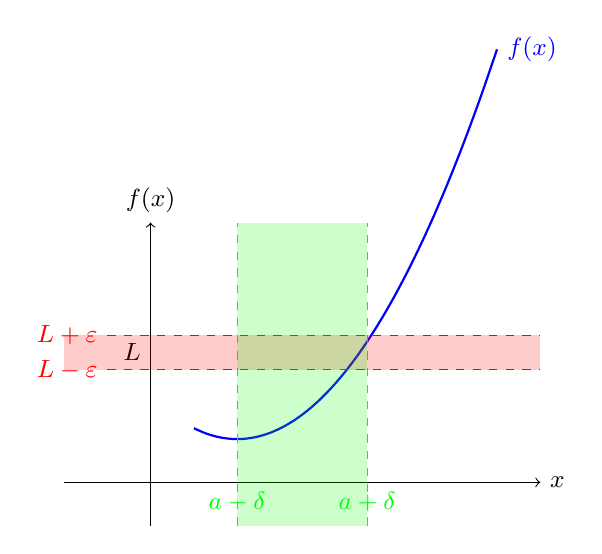
\begin{tikzpicture}[scale=1.1]
    % Axes
    \draw[->] (-1, 0) -- (4.5, 0) node[right] {\small $x$};
    \draw[->] (0, -0.5) -- (0, 3) node[above] {\small $f(x)$};

    % Function f(x)
    \draw[thick, blue] plot[domain=0.5:4, smooth] (\x, {0.5*(\x*\x - 2*\x + 2)}) 
        node[right] {\small $f(x)$};

    % Horizontal lines for L-epsilon and L+epsilon
    \draw[dashed, red] (-0.5, 1.3) -- (4.5, 1.3);
    \draw[dashed, red] (-0.5, 1.7) -- (4.5, 1.7);
    \node[left, red] at (-0.5, 1.3) {\small $L - \varepsilon$};
    \node[left, red] at (-0.5, 1.7) {\small $L + \varepsilon$};

    % Vertical lines for a-delta and a+delta
    \draw[dashed, green] (1, -0.5) -- (1, 3);
    \draw[dashed, green] (2.5, -0.5) -- (2.5, 3);
    \node[below, green] at (1, 0) {\small $a - \delta$};
    \node[below, green] at (2.5, 0) {\small $a + \delta$};

    % Mark L on y-axis
    \node[left] at (0, 1.5) {\small $L$};

    % Highlighted epsilon-delta region
    \fill[opacity=0.2, red] (-1, 1.3) rectangle (4.5, 1.7);
    \fill[opacity=0.2, green] (1, -0.5) rectangle (2.5, 3);
\end{tikzpicture}

\vspace{1cm}

\textbf{Cauchy: Sequences approaching \( a \) yield function values approaching \( L \)}

\vspace{0.5cm}

\begin{tikzpicture}[scale=1.1]
    % Horizontal axis (n)
    \draw[->] (-0.5,0) -- (10.5,0) node[right] {\( n \)};
    % Vertical axis (a_n)
    \draw[->] (0,-1) -- (0,4) node[above] {\( a_n \)};

    % Limit L
    \draw[dashed] (-0.5,2.5) -- (10.5,2.5) node[right] {\( L \)};
    % Epsilon bands
    \draw[dashed, red] (-0.5,3) -- (10.5,3) node[right] {\( L + \epsilon \)};
    \draw[dashed, red] (-0.5,2) -- (10.5,2) node[right] {\( L - \epsilon \)};

    % Threshold N
    \draw[dotted, thick] (5,-0.2) -- (5,4) node[above] {\( N \)};

    % Sequence points before N
    \foreach \x/\y in {1/0.8, 2/1.5, 3/3.8, 4/2.9} {
        \filldraw[blue] (\x,\y) circle (2pt);
    }
    % Sequence points after N
    \foreach \x/\y in {6/2.7, 7/2.55, 8/2.52, 9/2.505, 10/2.501} {
        \filldraw[green] (\x,\y) circle (2pt);
    }

    % Labels
    \node[below] at (5,0) {\( N \)};
    \node[left] at (0,2.5) {\( L \)};
    \node[align=left, right] at (7,1) {For \( n > N \),\\ \( |a_n - L| < \epsilon \)};
\end{tikzpicture}
\end{center}

\bigskip

This comparison captures the evolution: Cauchy described limits using sequences and behavior over time, while Weierstrass crystallized that idea into precise input-output constraints. The \(\varepsilon\)-\(\delta\) definition didn’t replace Cauchy—it made his intuition unbreakable.




To get a better sense of the mindset shift he triggered, imagine explaining limits to someone used to the old way of thinking—only this time, you’ve got Weierstrass’s \(\varepsilon\)-\(\delta\) toolkit in your back pocket.

\begin{quote}
{\ttfamily
\textbf{user1:} So what's all this noise about limits and $\varepsilon$-$\delta$? Isn’t a limit just... getting close to a number?

\textbf{user2:} Ah, that’s what we *used* to say. Then Weierstrass walked in with a flamethrower.

\textbf{user1:} Sounds dramatic.

\textbf{user2:} He thought infinitesimals were vague nonsense. So he nuked them and replaced the whole idea of limits with a definition using $\varepsilon$ and $\delta$.

\textbf{user1:} Okay, but what do they actually *do*?

\textbf{user2:} Think of $\varepsilon$ as your tolerance — how close you want $f(x)$ to be to the limit $L$.

\textbf{user1:} Got it. Tiny wiggle room around $L$.

\textbf{user2:} Exactly. And $\delta$ is the amount you're allowed to wiggle $x$ around $a$ to make sure $f(x)$ stays within that $\varepsilon$ window.

\textbf{user1:} So it's like: “If you want me to be *this* close to $L$, then you can’t move $x$ more than *that* far from $a$”?

\textbf{user2:} Boom. That’s the heart of the definition. For every $\varepsilon > 0$, there exists a $\delta > 0$ so that $|f(x) - L| < \varepsilon$ whenever $|x - a| < \delta$.

*** [cue Weierstrass sharpening chalk] ***

\textbf{user1:} That’s... actually kind of elegant?

\textbf{user2:} Right? It turned hand-wavy intuition into cold, hard math. Like a math proof fortress.

\textbf{user1:} And we never had to mention anything “infinitely small.”

\textbf{user2:} Nope. Weierstrass banned that from the premises. 
}
\end{quote}


\textbf{Why was this important?} Because math was getting away with vibes for way too long. Weierstrass wasn’t having it. By introducing the $\varepsilon$–$\delta$ definition, he eliminated the hand-wavy mysticism of infinitesimals and demanded logical receipts. No more "infinitely small changes" — just rock-solid, provable claims based on arbitrarily small (but still very real) quantities. The chat might’ve sounded dramatic, but this shift laid the groundwork for modern analysis — with rigor replacing intuition as the gold standard.


\subsection{Redefining Continuity: A Function That Never Breaks}

Using the \(\varepsilon\)-\(\delta\) framework, Weierstrass gave the first rigorous definition of continuity. A function \( f(x) \) is continuous at a point \( x = a \) if:

\vspace{0.5em}
\noindent\textbf{Definition.}
A function \( f(x) \) is \textbf{continuous at a point \( a \)} if:
\[
\forall \varepsilon > 0,\ \exists \delta > 0 \text{ such that if } |x - a| < \delta, \text{ then } |f(x) - f(a)| < \varepsilon.
\]
\vspace{1em}

This ensures that a function doesn't make sudden jumps. If you zoom in close enough, the values of the function remain arbitrarily close to \( f(a) \). Weierstrass provided a way to rigorously verify this, replacing geometric intuition with precise logic.

\begin{center}
\textbf{Weierstrass: Continuity via \(\varepsilon\)-\(\delta\)}

\vspace{0.5cm}

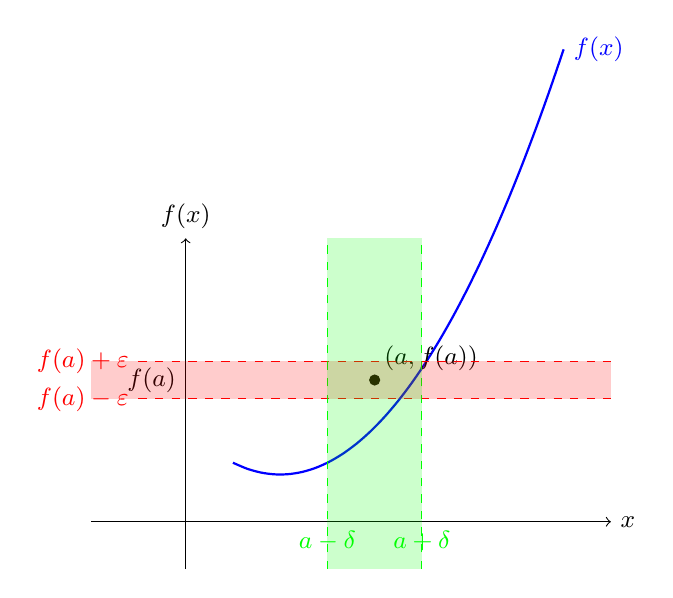
\begin{tikzpicture}[scale=1.2]
    % Axes
    \draw[->] (-1, 0) -- (4.5, 0) node[right] {\small $x$};
    \draw[->] (0, -0.5) -- (0, 3) node[above] {\small $f(x)$};

    % Function f(x) - continuous curve
    \draw[thick, blue] plot[domain=0.5:4, smooth] (\x, {0.5*(\x*\x - 2*\x + 2)}) 
        node[right] {\small $f(x)$};

    % Mark point a
    \filldraw[black] (2, 1.5) circle (1.5pt) node[above right] {\small $(a, f(a))$};

    % Horizontal lines for f(a)-epsilon and f(a)+epsilon
    \draw[dashed, red] (-0.5, 1.3) -- (4.5, 1.3);
    \draw[dashed, red] (-0.5, 1.7) -- (4.5, 1.7);
    \node[left, red] at (-0.5, 1.3) {\small $f(a) - \varepsilon$};
    \node[left, red] at (-0.5, 1.7) {\small $f(a) + \varepsilon$};

    % Vertical lines for a-delta and a+delta
    \draw[dashed, green] (1.5, -0.5) -- (1.5, 3);
    \draw[dashed, green] (2.5, -0.5) -- (2.5, 3);
    \node[below, green] at (1.5, 0) {\small $a - \delta$};
    \node[below, green] at (2.5, 0) {\small $a + \delta$};

    % Mark f(a)
    \node[left] at (0, 1.5) {\small $f(a)$};

    % Highlighted regions
    \fill[opacity=0.2, red] (-1, 1.3) rectangle (4.5, 1.7);
    \fill[opacity=0.2, green] (1.5, -0.5) rectangle (2.5, 3);
\end{tikzpicture}

\vspace{1cm}

\textbf{Cauchy: Continuity via Sequences}

\vspace{0.5cm}

A function \( f(x) \) is continuous at a point \( a \) if for every sequence \( x_n \to a \), the function values \( f(x_n) \to f(a) \).

\begin{tikzpicture}[scale=1.1]
    % Horizontal axis (n)
    \draw[->] (-0.5,0) -- (10.5,0) node[right] {\( n \)};
    % Vertical axis (f(x_n))
    \draw[->] (0,-1) -- (0,4) node[above] {\( f(x_n) \)};

    % Limit f(a)
    \draw[dashed] (-0.5,2.5) -- (10.5,2.5) node[right] {\( f(a) \)};
    % Epsilon bands
    \draw[dashed, red] (-0.5,3) -- (10.5,3) node[right] {\( f(a) + \epsilon \)};
    \draw[dashed, red] (-0.5,2) -- (10.5,2) node[right] {\( f(a) - \epsilon \)};

    % Threshold N
    \draw[dotted, thick] (5,-0.2) -- (5,4) node[above] {\( N \)};

    % Sequence points before N
    \foreach \x/\y in {1/1.2, 2/1.6, 3/3.1, 4/2.1} {
        \filldraw[blue] (\x,\y) circle (2pt);
    }
    % Sequence points after N
    \foreach \x/\y in {6/2.6, 7/2.55, 8/2.52, 9/2.505, 10/2.501} {
        \filldraw[green] (\x,\y) circle (2pt);
    }

    % Labels
    \node[below] at (5,0) {\( N \)};
    \node[left] at (0,2.5) {\( f(a) \)};
    \node[align=left, right] at (7,1) {For \( n > N \),\\ \( |f(x_n) - f(a)| < \epsilon \)};
\end{tikzpicture}
\end{center}

\bigskip

This side-by-side progression shows how Weierstrass reinforced and formalized Cauchy's ideas. Cauchy’s definition of continuity relied on the behavior of sequences approaching a point, while Weierstrass spelled out exactly how close inputs need to be to keep function values within a desired margin.

\begin{figure}[H]
\centering
\begin{tikzpicture}[every node/.style={font=\footnotesize}]

% Top-left panel: label under "Student" (left)
\comicpanel{0}{4}
  {Student}  % left name
  {Weierstrass}  % right name
  {So continuity just means you can draw the graph without lifting your pen, right?}
  {(-0.8,-0.45)}

% Top-right panel: label under "Weierstrass" (right)
\comicpanel{6.5}{4}
  {Student}
  {Weierstrass}
  {That is the worst definition I’ve ever heard.}
  {(0.8,-0.5)}

% Bottom-left panel: label under "Weierstrass" (left)
\comicpanel{0}{0}
  {Student}
  {Weierstrass}
  {From now on, continuity means: for every $\varepsilon > 0$, there exists a $\delta > 0$...}
  {(0.6,-0.5)}

% Bottom-right panel: label under "Student" (right)
\comicpanel{6.5}{0}
  {Student}
  {Weierstrasst}
  {Okay but... does this mean I still can't lift the pen?}
  {(-0.9,-0.6)}

\end{tikzpicture}
\caption{A 2x2 comic using reusable panel templates with programmable labels.}
\end{figure}






\subsection{Differentiability and the Crisis of Convergence}

Having made limits and continuity rigorous, Weierstrass turned to differentiation. The derivative,

\[
f'(x) = \lim_{\Delta x \to 0} \frac{f(x + \Delta x) - f(x)}{\Delta x}
\]

relied on the assumption that \( f(x) \) changed smoothly enough for this limit to exist.

Cauchy provided a sequence-based interpretation: if \( h_n \to 0 \), then the difference quotients
\[
\frac{f(x + h_n) - f(x)}{h_n}
\]
should converge to the same value, regardless of the sequence, for the derivative to exist.

Weierstrass formalized this further with an \( \varepsilon \)-\( \delta \) definition of differentiability:

\vspace{0.5em}
\noindent\textbf{Definition.}
A function \( f(x) \) is \textbf{differentiable at a point \( x = c \)} if there exists a real number \( L \) such that:
\[
\forall \varepsilon > 0,\ \exists \delta > 0 \text{ such that if } 0 < |h| < \delta,\ \left|\frac{f(c + h) - f(c)}{h} - L\right| < \varepsilon.
\]
\vspace{1em}

This definition ensures that the difference quotients not only approach some value but do so in a controlled and uniform way as \( h \to 0 \).

\begin{center}
\textbf{Weierstrass: Differentiability via \( \varepsilon \)-\( \delta \)}

\vspace{0.5cm}

\begin{tikzpicture}[scale=1.2]
    % Draw axes
    \draw[->] (-1,0) -- (7,0) node[right] {\( x \)};
    \draw[->] (0,-1) -- (0,5) node[above] {\( f(x) \)};

    % Smooth function (Differentiable)
    \draw[thick, blue, domain=0.5:3.5, smooth] plot (\x, {0.5*\x*\x - 0.8*\x + 2});
    \filldraw[black] (2,2) circle (2pt) node[above left] {\( (c, f(c)) \)};
    \draw[dashed, green] (0,1.2) -- (4,2.8);  % Tangent line
    \node[left] at (0.5,1.5) {\footnotesize Tangent exists};

    % Labels
    \node[below] at (2,0) {\( c \)};
\end{tikzpicture}

\vspace{1cm}

\textbf{Cauchy: Differentiability via Sequences}

\vspace{0.5cm}

A function \( f(x) \) is differentiable at \( x = c \) if for every sequence \( h_n \to 0 \) (with \( h_n \neq 0 \)), the difference quotient sequence
\[
\frac{f(c + h_n) - f(c)}{h_n}
\]
converges to the same value \( L \).

\begin{tikzpicture}[scale=1.1]
    % Horizontal axis (n)
    \draw[->] (-0.5,0) -- (10.5,0) node[right] {\( n \)};
    % Vertical axis (difference quotient)
    \draw[->] (0,-1) -- (0,4) node[above] {\( \frac{f(c+h_n) - f(c)}{h_n} \)};

    % Limit L
    \draw[dashed] (-0.5,2.5) -- (10.5,2.5) node[right] {\( L \)};
    % Epsilon bands
    \draw[dashed, red] (-0.5,3) -- (10.5,3) node[right] {\( L + \epsilon \)};
    \draw[dashed, red] (-0.5,2) -- (10.5,2) node[right] {\( L - \epsilon \)};

    % Threshold N
    \draw[dotted, thick] (5,-0.2) -- (5,4) node[above] {\( N \)};

    % Sequence points before N
    \foreach \x/\y in {1/1.2, 2/1.9, 3/3.1, 4/2.1} {
        \filldraw[blue] (\x,\y) circle (2pt);
    }
    % Sequence points after N
    \foreach \x/\y in {6/2.6, 7/2.55, 8/2.52, 9/2.505, 10/2.501} {
        \filldraw[green] (\x,\y) circle (2pt);
    }

    % Labels
    \node[below] at (5,0) {\( N \)};
    \node[left] at (0,2.5) {\( L \)};
    \node[align=left, right] at (7,1) {For \( n > N \),\\ \( \left| \frac{f(c+h_n) - f(c)}{h_n} - L \right| < \epsilon \)};
\end{tikzpicture}
\end{center}

\bigskip

These two views—Weierstrass with \( \varepsilon \)-\( \delta \), and Cauchy with sequences—offered converging paths to the same rigorous concept: differentiability. But the journey didn’t end there. As Weierstrass would show, even continuous functions can behave wildly, and not all of them are differentiable.


\begin{figure}[H]
\centering
\begin{tikzpicture}[every node/.style={font=\footnotesize}]

% Top-left panel
\comicpanel{0}{4}
  {Cauchy}  % left name
  {Weierstrass}  % right name
  {If every sequence $h_n \to 0$ gives the same limit, the derivative exists. Simple!}
  {(-1.1,-0.45)}

% Top-right panel
\comicpanel{6.5}{4}
  {Cauchy}
  {Weierstrass}
  {And what if one sequence misbehaves? We need $\varepsilon$ and $\delta$ to keep them all in line.}
  {(1,-0.5)}

% Bottom-left panel
\comicpanel{0}{0}
  {Cauchy}
  {Weierstrass}
  {So you're replacing intuition with a security system?}
  {(-0.9,-0.5)}

% Bottom-right panel
\comicpanel{6.5}{0}
  {Cauchy}
  {Weierstrass}
  {Exactly. Math isn’t safe until everything is bounded.}
  {(0.2,-0.6)}

\end{tikzpicture}
\caption{A 2x2 comic where Cauchy and Weierstrass discuss differentiability.}
\end{figure}










\subsection{The Birth of Mathematical Monsters: Weierstrass’s Nowhere-Differentiable Function}

With Weierstrass’ \(\varepsilon\)-\(\delta\) definitions of limits and continuity, it seemed like functions had been fully tamed.

\begin{quote}
\textbf{If a function was continuous, we could analyze it.}\\
\textbf{If a function was differentiable, we could describe its rate of change.}\\
\textbf{If a function was integrable, we could measure areas under it.}
\end{quote}

But what if a function didn’t behave as expected? What if smooth methods, carefully developed through centuries of calculus, suddenly failed?

\begin{center}
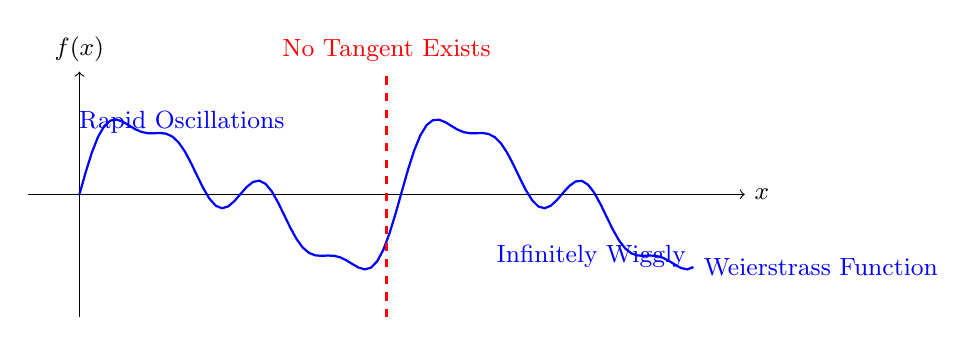
\begin{tikzpicture}[scale=1.3]

    % Axes
    \draw[->] (-0.5, 0) -- (6.5, 0) node[right] {\small $x$};
    \draw[->] (0, -1.2) -- (0, 1.2) node[above] {\small $f(x)$};

    % Plot an approximation of the Weierstrass function using a sum of cosines
    \draw[thick, blue, domain=0:6, samples=100] 
        plot (\x, {0.6*sin(2*\x r) + 0.3*sin(4*\x r) + 0.15*sin(8*\x r)}) 
        node[right] {\small Weierstrass Function};

    % Tangent attempt at x=3 (fails due to infinite oscillations)
    \draw[thick, dashed, red] (3, -1.2) -- (3, 1.2);
    \node[red, above] at (3, 1.2) {\small No Tangent Exists};

    % Labels for oscillatory behavior
    \node[blue] at (1, 0.7) {\small Rapid Oscillations};
    \node[blue] at (5, -0.6) {\small Infinitely Wiggly};

\end{tikzpicture}
\end{center}

Functions could behave badly at a \textbf{few isolated points}, but if a function was \textbf{continuous everywhere}, surely it must be differentiable \textbf{almost everywhere}—or at least well-behaved in most cases.

Weierstrass shattered this intuition. He constructed a function that was \textbf{continuous everywhere} but \textbf{differentiable nowhere}—a function that wiggled so wildly at every single point that a tangent line could never be defined.

\[
W(x) = \sum_{n=0}^{\infty} a^n \cos(b^n \pi x)
\]

where \( 0 < a < 1 \) and \( b \) is a positive odd integer chosen so that the function oscillates ever more rapidly as \( n \to \infty \). Unlike smooth curves that flatten out under magnification, \textbf{this function remained infinitely jagged at every scale}.




\begin{figure}[H]
\centering
\begin{tikzpicture}[every node/.style={font=\footnotesize}]

% Top-left panel
\comicpanel{0}{4}
  {Mathematician}
  {Weierstrass}
  {If a function is continuous everywhere, surely it's differentiable somewhere... right?}
  {(-0.7,-0.5)}

% Top-right panel
\comicpanel{6.5}{4}
  {Mathematician}
  {Weierstrass}
  {I built one that’s continuous everywhere and differentiable nowhere.}
  {(0.4,-0.4)}

% Bottom-left panel
\comicpanel{0}{0}
  {Mathematician}
  {Weierstrass}
  {That’s not a function. That’s a fractal having a panic attack.}
  {(-0.9,-0.55)}

% Bottom-right panel
\comicpanel{6.5}{0}
  {Mathematician}
  {Weierstrass}
  {Exactly. And it obeys every rule of analysis. Sleep well.}
  {(0.1,-0.6)}

\end{tikzpicture}
\caption{A 2x2 comic on Weierstrass’s nowhere-differentiable function.}
\end{figure}


\subsection{Mathematicians Were Horrified—And Frankly, It Was Hilarious}

\begin{quote}
    \textit{"Functions like these are monsters!"} — Charles Hermite  
\end{quote}

Weierstrass didn’t just break the rules; he set them on fire and then lectured about why the flames were actually a valid mathematical construct.  

His infamous function wasn’t just counterintuitive: it was an affront to everything respectable mathematicians held dear. If even \textbf{continuous functions} could behave like this, what other nightmares were lurking in analysis? It was the mathematical equivalent of realizing your childhood home had been built on an active sinkhole.  

Naturally, this kind of chaos did not go over well.  

\begin{itemize}
    \item Leopold Kronecker was so offended he basically staged a one-man intervention for mathematics, insisting that numbers should only exist if they were explicitly constructed.  
    \item Charles Hermite took one look at Weierstrass’s function and immediately declared it a "monster," presumably before going home to clutch his calculus textbooks and whisper reassuring words to them.  
    \item And the rest of the mathematical world? Somewhere between denial and existential dread.  
\end{itemize}

But here’s the thing: Weierstrass wasn’t wrong. His function was continuous everywhere but differentiable nowhere, a horrifying paradox wrapped in rigorous proof. And when the dust settled, it became impossible to unsee.  

The comforting notion that continuous functions were always well-behaved? Gone.  

The idea that calculus was built on solid ground? Please.  

Weierstrass had delivered an inconvenient truth: the foundation of analysis had cracks, and everyone had just been politely ignoring them.  



\begin{figure}[H]
\centering
\begin{tikzpicture}[every node/.style={font=\footnotesize}]

% Top-left panel
\comicpanel{0}{4}
  {Hermite}
  {Weierstrass}
  {This function is continuous but not differentiable anywhere.}
  {(0.5,-0.45)}

% Top-right panel
\comicpanel{6.5}{4}
  {Hermite}
  {Weierstrass}
  {That’s not a function. That’s a monster.}
  {(-0.8,-0.5)}

% Bottom-left panel
\comicpanel{0}{0}
  {Kronecker}
  {Weierstrass}
  {If I can’t construct it, it shouldn’t exist. I'm banning it from mathematics.}
  {(-0.9,-0.5)}

% Bottom-right panel
\comicpanel{6.5}{0}
  {Weierstrass}
  {Everyone}
  {It’s real, it’s legal, and it terrifies everyone.}
  {(0.4,-0.5)}

\end{tikzpicture}
\caption{A 2x2 comic about the horrified reaction to Weierstrass’s nowhere-differentiable function.}
\end{figure}
